% ------------------------------------------------------------------------------
% TYPO3 CMS 8.3 - What's New - Chapter "Introduction" (Serbian Version)
%
% @author	Michael Schams <schams.net>
% @license	Creative Commons BY-NC-SA 3.0
% @link		http://typo3.org/download/release-notes/whats-new/
% @language	Serbian
% ------------------------------------------------------------------------------
% LTXE-CHAPTER-UID:		7fdf26cc-362160ab-d6c8b905-19722b20
% LTXE-CHAPTER-NAME:	Introduction
% ------------------------------------------------------------------------------

\section{Uvod}
\begin{frame}[fragile]
	\frametitle{Uvod}

	\begin{center}\huge{Uvod}\end{center}
	\begin{center}\huge{\color{typo3darkgrey}\textbf{Cinjenice}}\end{center}

\end{frame}

% ------------------------------------------------------------------------------
% LTXE-SLIDE-START
% LTXE-SLIDE-UID:		410ba6bc-f8591599-0388ed17-3f7c3890
% LTXE-SLIDE-ORIGIN:	ca3596df-e5f14953-556d9c5f-a8a689fe English
% LTXE-SLIDE-TITLE:		TYPO3 CMS 8.2 and 8.3 - The Facts
% ------------------------------------------------------------------------------
\begin{frame}[fragile]
	\frametitle{Uvod}
	\framesubtitle{TYPO3 CMS 8.2 i 8.3 - Cinjenice}

	\textbf{TYPO3 CMS 8.2}
	\begin{itemize}
		\item Datum objavljivanja: 5. juli 2016.
		\item Tip objavljivanja: "Brza objava" ("Sprint Release")
		\item Slogan: Unapredjenja
	\end{itemize}

	\vspace{0.6cm}

	\textbf{TYPO3 CMS 8.3}
	\begin{itemize}
		\item Datum objavljivanja: 30. avgust 2016.
		\item Tip objavljivanja: "Brza objava" ("Sprint Release")
		\item Slogan: Administracija korisnickog interfejsa na steroidima
	\end{itemize}

%	\begin{figure}
%		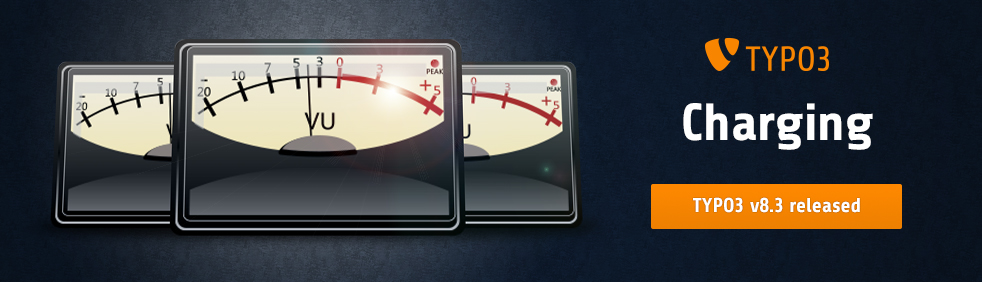
\includegraphics[width=0.95\linewidth]{Introduction/typo3cms83-banner.jpg}
%	\end{figure}

\end{frame}

% ------------------------------------------------------------------------------
% LTXE-SLIDE-START
% LTXE-SLIDE-UID:		0324fc36-0de4d9d8-39a7a03a-a854e5bd
% LTXE-SLIDE-ORIGIN:	1be10378-6e990dd6-2cca609a-c778c43c English
% LTXE-SLIDE-TITLE:		System Requirements
% ------------------------------------------------------------------------------
\begin{frame}[fragile]
	\frametitle{Uvod}
	\framesubtitle{Sistemski zahtevi}

	\begin{itemize}
		\item PHP:\tabto{2.2cm}verzija 7
		\item MySQL:\tabto{2.2cm}verzija  5.5 do 5.7
		\item Prostor na disku:\tabto{2.2cm}min 200 MB
		\item PHP podesavanja::

			\begin{itemize}
				\item \texttt{memory\_limit} >= 128M
				\item \texttt{max\_execution\_time} >= 240s
				\item \texttt{max\_input\_vars} >= 1500
				\item opcija za kompajliranje \texttt{-}\texttt{-disable-ipv6} \underline{se ne sme koristiti} 
			\end{itemize}

		\item Administratorski interfejs zahteva Microsoft Internet Explorer 11 ili noviji, 
			Microsoft Edge, Google Chrome, Firefox, Safari 
			ili bilo koji drugi moderni kompatibilni pretrazivac

	\end{itemize}

\end{frame}

% ------------------------------------------------------------------------------
% LTXE-SLIDE-START
% LTXE-SLIDE-UID:		f1090dd3-f2b55fc0-89f57b73-33bc6a8c
% LTXE-SLIDE-ORIGIN:	ed8e8933-d90001c7-f7548bd3-80e549cb English
% LTXE-SLIDE-TITLE:		Development And Release Timeline
% ------------------------------------------------------------------------------
\begin{frame}[fragile]
	\frametitle{Uvod}
	\framesubtitle{Vreme razvoja i datumi objavljivanja}

	\begin{figure}
		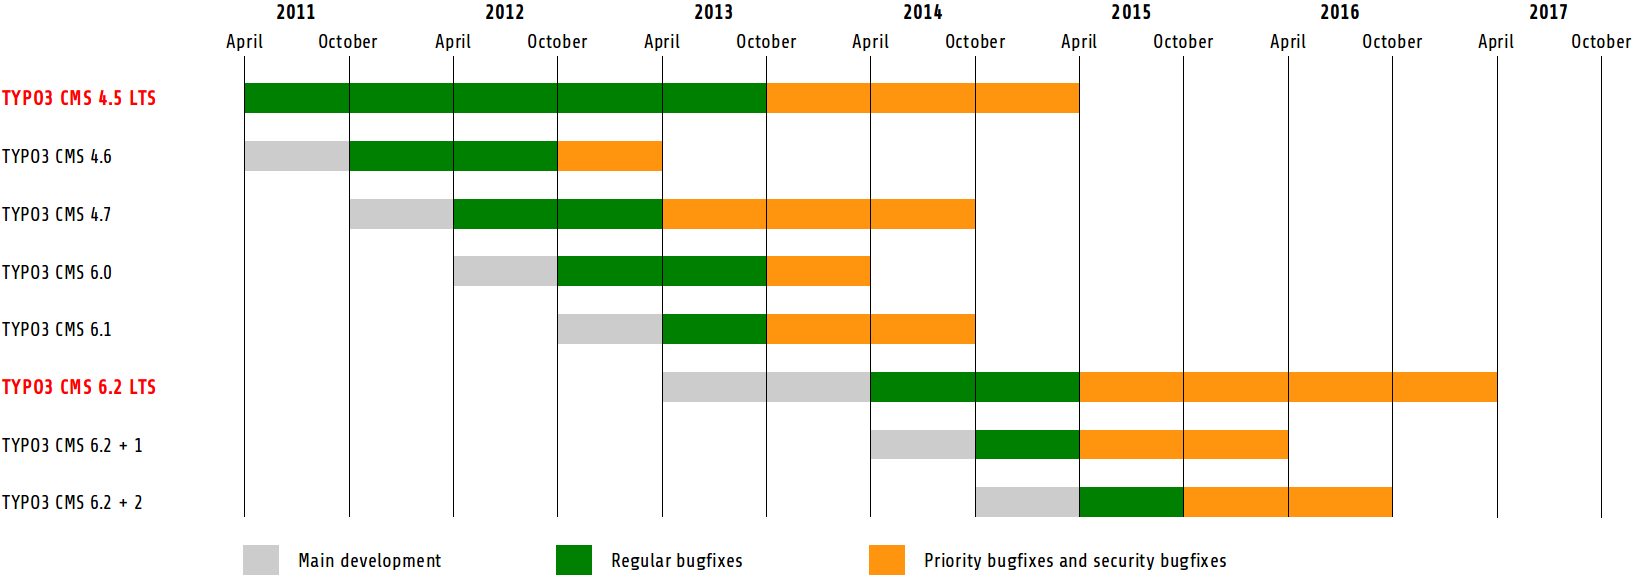
\includegraphics[width=1\linewidth]{Introduction/ReleaseAgenda.png}
	\end{figure}

\end{frame}

% ------------------------------------------------------------------------------
% LTXE-SLIDE-START
% LTXE-SLIDE-UID:		32b19940-3509a17c-81db1526-5509f851
% LTXE-SLIDE-ORIGIN:	01225efb-e9fdbaff-726e5fed-5b7f0003 English
% LTXE-SLIDE-TITLE:		TYPO3 CMS Roadmap
% ------------------------------------------------------------------------------
\begin{frame}[fragile]
	\frametitle{Uvod}
	\framesubtitle{TYPO3 CMS plan}

	Predvidjeni datumi objavljivanja i njihov osnovni fokus:

	\begin{itemize}

		\item v8.0 \tabto{1.1cm}22/Mar/2016\tabto{3.4cm}Finalna podesavanja
		\item v8.1 \tabto{1.1cm}03/May/2016\tabto{3.4cm}Integracija Cloud-a
		\item
			\begingroup
				\color{typo3orange}
					v8.2 \tabto{1.1cm}05/Jul/2016\tabto{3.4cm}Unapredjenja
			\endgroup
		\item
			\begingroup
				\color{typo3orange}
					v8.3 \tabto{1.1cm}30/Aug/2016\tabto{3.4cm}Administracija korisnickog interfejsa na steroidima
			\endgroup
		\item v8.4 \tabto{1.1cm}18/Oct/2016\tabto{3.4cm}\textit{bice odredjeno}
		\item v8.5 \tabto{1.1cm}20/Dec/2016\tabto{3.4cm}Podrska za integratore
		\item v8.6 \tabto{1.1cm}14/Feb/2017\tabto{3.4cm}\textit{bice odredjeno}
		\item v8.7 \tabto{1.1cm}04/Apr/2017\tabto{3.4cm}Priprema za LTS

	\end{itemize}

	\smaller
		\url{https://typo3.org/typo3-cms/roadmap/}\newline
		\url{https://typo3.org/news/article/kicking-off-typo3-v8-development/}
	\normalsize

\end{frame}

% ------------------------------------------------------------------------------
% LTXE-SLIDE-START
% LTXE-SLIDE-UID:		d5304623-2a0d32f4-b6bdfcf7-64a55e24
% LTXE-SLIDE-ORIGIN:	793cc944-52bccf17-ba7c4c9c-661e8993 English
% LTXE-SLIDE-TITLE:		Installation
% ------------------------------------------------------------------------------
\begin{frame}[fragile]
	\frametitle{Uvod}
	\framesubtitle{Instalacija}

	\begin{itemize}
		\item Zvanicna procedura za instalaciju na Linux/Mac OS X\newline
			(DocumentRoot na primer \texttt{/var/www/site/htdocs}):
		\begin{lstlisting}
			$ cd /var/www/site
			$ wget --content-disposition get.typo3.org/8.3
			$ tar xzf typo3_src-8.3.0.tar.gz
			$ cd htdocs
			$ ln -s ../typo3_src-8.3.0 typo3_src
			$ ln -s typo3_src/index.php
			$ ln -s typo3_src/typo3
			$ touch FIRST_INSTALL
		\end{lstlisting}

		\item Simbolicki linkovi (Symbolic links) na Microsoft Windows:

			\begin{itemize}
				\item Koristiti \texttt{junction} za Windows XP/2000
				\item Koristiti \texttt{mklink} za Windows Vista i Windows 7
			\end{itemize}

	\end{itemize}
\end{frame}

% ------------------------------------------------------------------------------
% LTXE-SLIDE-START
% LTXE-SLIDE-UID:		5d540601-cab0e0df-31bcb882-d3c76d50
% LTXE-SLIDE-ORIGIN:	4c0c3586-154241f9-4c859652-03bcc92e English
% LTXE-SLIDE-TITLE:		Upgrade to TYPO3 CMS 7
% ------------------------------------------------------------------------------
\begin{frame}[fragile]
	\frametitle{Uvod}
	\framesubtitle{Nadogradnja na TYPO3 CMS 8.x}

	\begin{itemize}
		\item Nadogradnja je moguca samo sa TYPO3 CMS 7.6 LTS
		\item TYPO3 CMS < 7.6 LTS bi prvo trebalo nadograditi na TYPO3 CMS 7.6 LTS
	\end{itemize}

	\begin{itemize}

		\item Upsutstvo za nadogradnju:\newline
			\smaller\url{http://wiki.typo3.org/Upgrade#Upgrading_to_8.3}\normalsize
		\item Zvanicni TYPO3 vodic "TYPO3 Installation and Upgrading":
			\smaller\url{http://docs.typo3.org/typo3cms/InstallationGuide}\normalsize
		\item Opsti pristup:
			\begin{itemize}
				\item Proveriti minimalne sistemske zahte \small(PHP, MySQL, etc.)
				\item Proveriti \textbf{deprecation\_*.log} u staroj TYPO3 instanci
				\item Nadograditi sva prosirenja na najnoviju verziju
				\item Postaviti nove fajlove i pokrenuti Install Tool -> Upgrade Wizard
				\item Proveriti startup modul za administratore (opciono)
			\end{itemize}
	\end{itemize}

\end{frame}

% ------------------------------------------------------------------------------

% ------------------------------------------------------------------------------
% LTXE-SLIDE-START
% LTXE-SLIDE-UID:		79a2e31e-c01fa78f-1c5bc81c-b67a3b66
% LTXE-SLIDE-ORIGIN:	36c478bf-991c3c9c-1b55ed59-ee1ad72e English
% LTXE-SLIDE-TITLE:		PHP Version 7
% ------------------------------------------------------------------------------
\begin{frame}[fragile]
	\frametitle{Uvod}
	\framesubtitle{PHP verzija 7}

	\begin{itemize}

		\item PHP 7.0 je minimalni zahtev za TYPO3 CMS 8.x
		\item TYPO3 ce podrzavati sve dolazece verzije PHP 7 kako budu izlazile
		\item Ovo unapredjenje verzije donelo je znacajno poboljsanje u performansama celog sistema

		\item Ne samo da ce urednici primetiti pokretniji interfejs, vec su i na korisnickom interfejsu 
			novi zapisi na kesiranim stranama generisani za manje od 7 milisekundi,
			sto je priblizno 40\% brze u odnosu na potpuno istu internet stranicu sa PHP verzijom 5.5

		\item Takodje smo poceli koristiti nova svojstva iz ove PHP verzije, 
			na primer cryptographically secure pseudo-random generatori su vec u funkciji

	\end{itemize}

\end{frame}

% ------------------------------------------------------------------------------
